\documentclass{article}  % Define la clase del documento.

% Paquetes de idioma y codificación
\usepackage[utf8]{inputenc}
\usepackage[T1]{fontenc}
\usepackage[spanish]{babel}  % Ajusta el idioma del documento a español.
\usepackage{tabularx}  % Permite la creación de tablas con ancho ajustable.

% Paquete de geometría para configurar márgenes y tamaño de papel
\usepackage[letterpaper, margin=3cm]{geometry}

% Paquetes de tipografía
\usepackage{mathptmx}    % Usa Times New Roman como fuente.
\usepackage{microtype}   % Mejora la justificación del texto.

% Paquetes para manejo de colores y gráficos
\usepackage{xcolor}      % Define y utiliza colores.
\usepackage{graphicx}    % Permite la inserción de imágenes.
\usepackage{tikz}        % Creación de gráficos vectoriales.
\usepackage{amsfonts}


% Configuración de enlaces y referencias cruzadas
\usepackage{hyperref}
\hypersetup{
    colorlinks   = true,
    linkcolor    = darkblue,
    citecolor    = black,
    filecolor    = blue,
    urlcolor     = blue
}

\usepackage{media9} % Permite la inserción de multimedia.

% Paquetes para la mejora visual de tablas y figuras
\usepackage{booktabs}    % Para tablas de alta calidad.
\usepackage{float}       % Controla la posición de figuras y tablas.

% Paquete para la personalización de códigos fuente
\usepackage{listings}
\lstset{
    literate=
    {á}{{\'a}}1 {é}{{\'e}}1 {í}{{\'i}}1 {ó}{{\'o}}1 {ú}{{\'u}}1
    {Á}{{\'A}}1 {É}{{\'E}}1 {Í}{{\'I}}1 {Ó}{{\'O}}1 {Ú}{{\'U}}1
    {ñ}{{\~n}}1 {Ñ}{{\~N}}1 {ü}{{\"u}}1 {Ü}{{\"U}}1,
    backgroundcolor=\color{backcolour},
    commentstyle=\color{codegreen},
    keywordstyle=\color{codepurple},
    numberstyle=\tiny\color{codegray},
    stringstyle=\color{red},
    basicstyle=\ttfamily\small,
    breakatwhitespace=false,
    breaklines=true,
    captionpos=b,
    keepspaces=true,
    numbers=left,
    numbersep=5pt,
    showspaces=false,
    showstringspaces=false,
    showtabs=false,
    tabsize=2,
    language=TeX,
    morecomment=[l]\#,
    frame=single,
    rulecolor=\color{black}
}

% Definición de colores al estilo Visual Studio Code
\definecolor{darkblue}{rgb}{0.0, 0.0, 0.55}  % Enlaces
\definecolor{codegreen}{rgb}{0.25, 0.49, 0.48}  % Comentarios
\definecolor{codegray}{rgb}{0.5, 0.5, 0.5}  % Números y anotaciones
\definecolor{codepurple}{rgb}{0.58, 0, 0.82}  % Palabras clave
\definecolor{backcolour}{rgb}{0.95, 0.95, 0.92}  % Fondo de código

% Configuraciones de párrafo y matemáticas
\usepackage{amsmath}
\usepackage{parskip}    % Espaciado entre párrafos.
\usepackage{ragged2e}   % Justificación mejorada.

% Configuración de secciones y encabezados
\usepackage{titlesec}
\titleclass{\part}{top}
\titleformat{\part}[display]
  {\normalfont\huge\bfseries\centering}{\thepart}{40pt}{\Huge}
\titlespacing*{\part}{0pt}{-60pt}{10pt}
\titleformat{\part}
  {\normalfont\huge\bfseries}{}{0pt}{}
\titleformat{\part}[display]
  {\normalfont\huge\bfseries}{}{0pt}{}
  [\thispagestyle{fancy}]

% Encabezado y pie de página
\usepackage{fancyhdr}
\pagestyle{fancy}
\fancyhf{}
\fancyhead[L]{\raisebox{0.20cm}{\textbf{Dinamica Prueba 1}}}
\fancyhead[R]{\raisebox{0.1cm}{
\includegraphics[width=0.25\linewidth]{LOGO_UNIVERSIDAD.jpg}}}
\fancyhead[C]{\rule{\textwidth}{0.6pt}}
\fancyfoot[C]{\rule{\textwidth}{0.6pt}}
\fancyfoot[R]{\raisebox{-1.5\baselineskip}{\thepage}}
\renewcommand{\headrulewidth}{0pt}
\renewcommand{\footrulewidth}{0pt}

% Geometría avanzada
\geometry{
  top=3.5cm,
  bottom=2.5cm,
  headheight=2.5cm
}

% Bibliografía
\usepackage{natbib}
\bibliographystyle{unsrtnat}

\begin{document}

%---------------------------------------- PORTADA ----------------------------------------
\begin{titlepage}
\newcommand{\HRule}{\rule{\linewidth}{0.5mm}} 
\center

\includegraphics[width=10cm]{LOGO_UNIVERSIDAD.jpg}\\
\vspace{3cm}
\HRule \\[0.4cm]
{ \huge \bfseries Prueba 1}\\[0.4cm]
{ \huge \bfseries Dinamica}\\[0.4cm]
\HRule \\[1.5cm]
\vspace{7.5cm}
\begin{center}

    \Large Lukas Wolff Casanova\\
\end{center}
\vspace{0.5cm}
{\large \textbf{\today}}\\[2cm]
\end{titlepage}



\newpage
\setcounter{page}{1}

%---------------------------------------- CONTENIDO ----------------------------------------

\section{Introduccion al sistema dinamico}

Un sistema dinamico de un DOF, se puede describir por la siguiente ecuacion:

\begin{equation}
    m \ddot{x} + c \dot{x} + kx = p(t)
\end{equation}

Donde:

\begin{equation}
    \int_{t_0}^{t} [m \ddot{u}(t)] \dot{u}(t) dt = \Delta E_k = \text{Variacion de la energia cinetica}
\end{equation}

\begin{equation}
    \int_{t_0}^{t} p(t) \dot{u}(t) dt = \int_{u_0}^{u} p(t) du = W_{ext} = \text{Trabajo externo}
\end{equation}

\begin{equation}
    \int_{t_0}^{t} k u(t) \dot{u}(t) dt = \Delta U_int = \text{Variacion de la energia interna}
\end{equation}

\begin{equation}
    \int_{t_0}^{t} c \dot{u^2}(t) dt = W_{dis}
\end{equation}

Por lo tanto, la ecuacion de movimiento se puede escribir como:

\begin{equation}
   \Delta E_k + \Delta U_int= W_{ext} - W_{dis} + {E_{k-t0} + U_{int-t0}} 
\end{equation}


\section{Inercias}

La inercia de un cuerpo largo respecto a un eje de rotacion es:
\begin{equation}
    I = \frac{mL^2}{12}
\end{equation}



\newpage
\section{Sistema no armortiguado de un DOF}

La ecuacion base de este sistema es:

\begin{equation}
    m \ddot{x} + kx = p(t)
\end{equation}

Se define la frecuencia angular natural como

\begin{equation}
    \omega_n = \sqrt{\frac{k}{m}} \quad f_n = \frac{\omega_n}{2\pi} \quad T_n = \frac{1}{f_n} 
\end{equation}

Luego, la ecuacion general del sistema se escribe como:

\begin{equation}
    u(t) = u_h(t) + u_p(t)
\end{equation}

Donde la homogenea corresponde al caso que $p(t) = 0$:

\begin{equation}
    u_h(t) = A \cos(\omega_n t) + B \sin(\omega_n t)
\end{equation}

Donde para determinar las constantes A y B, se utilizan las condiciones iniciales, por ejemplo:

\begin{equation}
    u(0) = u_0 \quad \text{y} \quad \ddot{u}(0) = \ddot{u_0}
\end{equation}

Por lo tanto, se obtiene (con condiciones iniciales $u_0 y \dot{u_0}$):

\begin{equation}
    A = \frac{\dot{u_0}}{\omega_n} \quad \text{y} \quad B = u_0
\end{equation}

Luego se pueden definir los siguientes terminos:
\begin{equation}
    \rho = \sqrt{u_0^2 + (\frac{\dot{u_0}}{\omega_n})^2} \quad \text{y} \quad \phi = \tan^{-1}(\frac{\dot{u_0}}{u_0 \omega_n})
\end{equation}

En realidad:

\begin{equation}
    \rho = \sqrt{A^2 + B^2} \quad \text{y} \quad \phi = \tan^{-1}(\frac{B}{A})
\end{equation}

Donde $\rho$ es la amplitud y $\phi$ es la fase. Por lo tanto, la ecuacion de movimiento se puede escribir como:

\begin{equation}
    u(t) = \rho \cos(\omega_n t - \phi)
\end{equation}

\begin{equation}
    \dot{u}(t) = -\rho \omega_n \sin(\omega_n t - \phi)
\end{equation}

\begin{equation}
    \ddot{u}(t) = -\rho \omega_n^2 \cos(\omega_n t - \phi)
\end{equation}

Ademas, se puede calcular el $T_{max}$ como:

\begin{equation}
    T_{max} = \frac{\phi}{\omega_n} + \frac{2\pi}{\omega_n} 
\end{equation}

Donde el $2\pi$ corresponde por cada ciclo.

Algunos ejemplos son:

\begin{figure}[H]
    \centering
    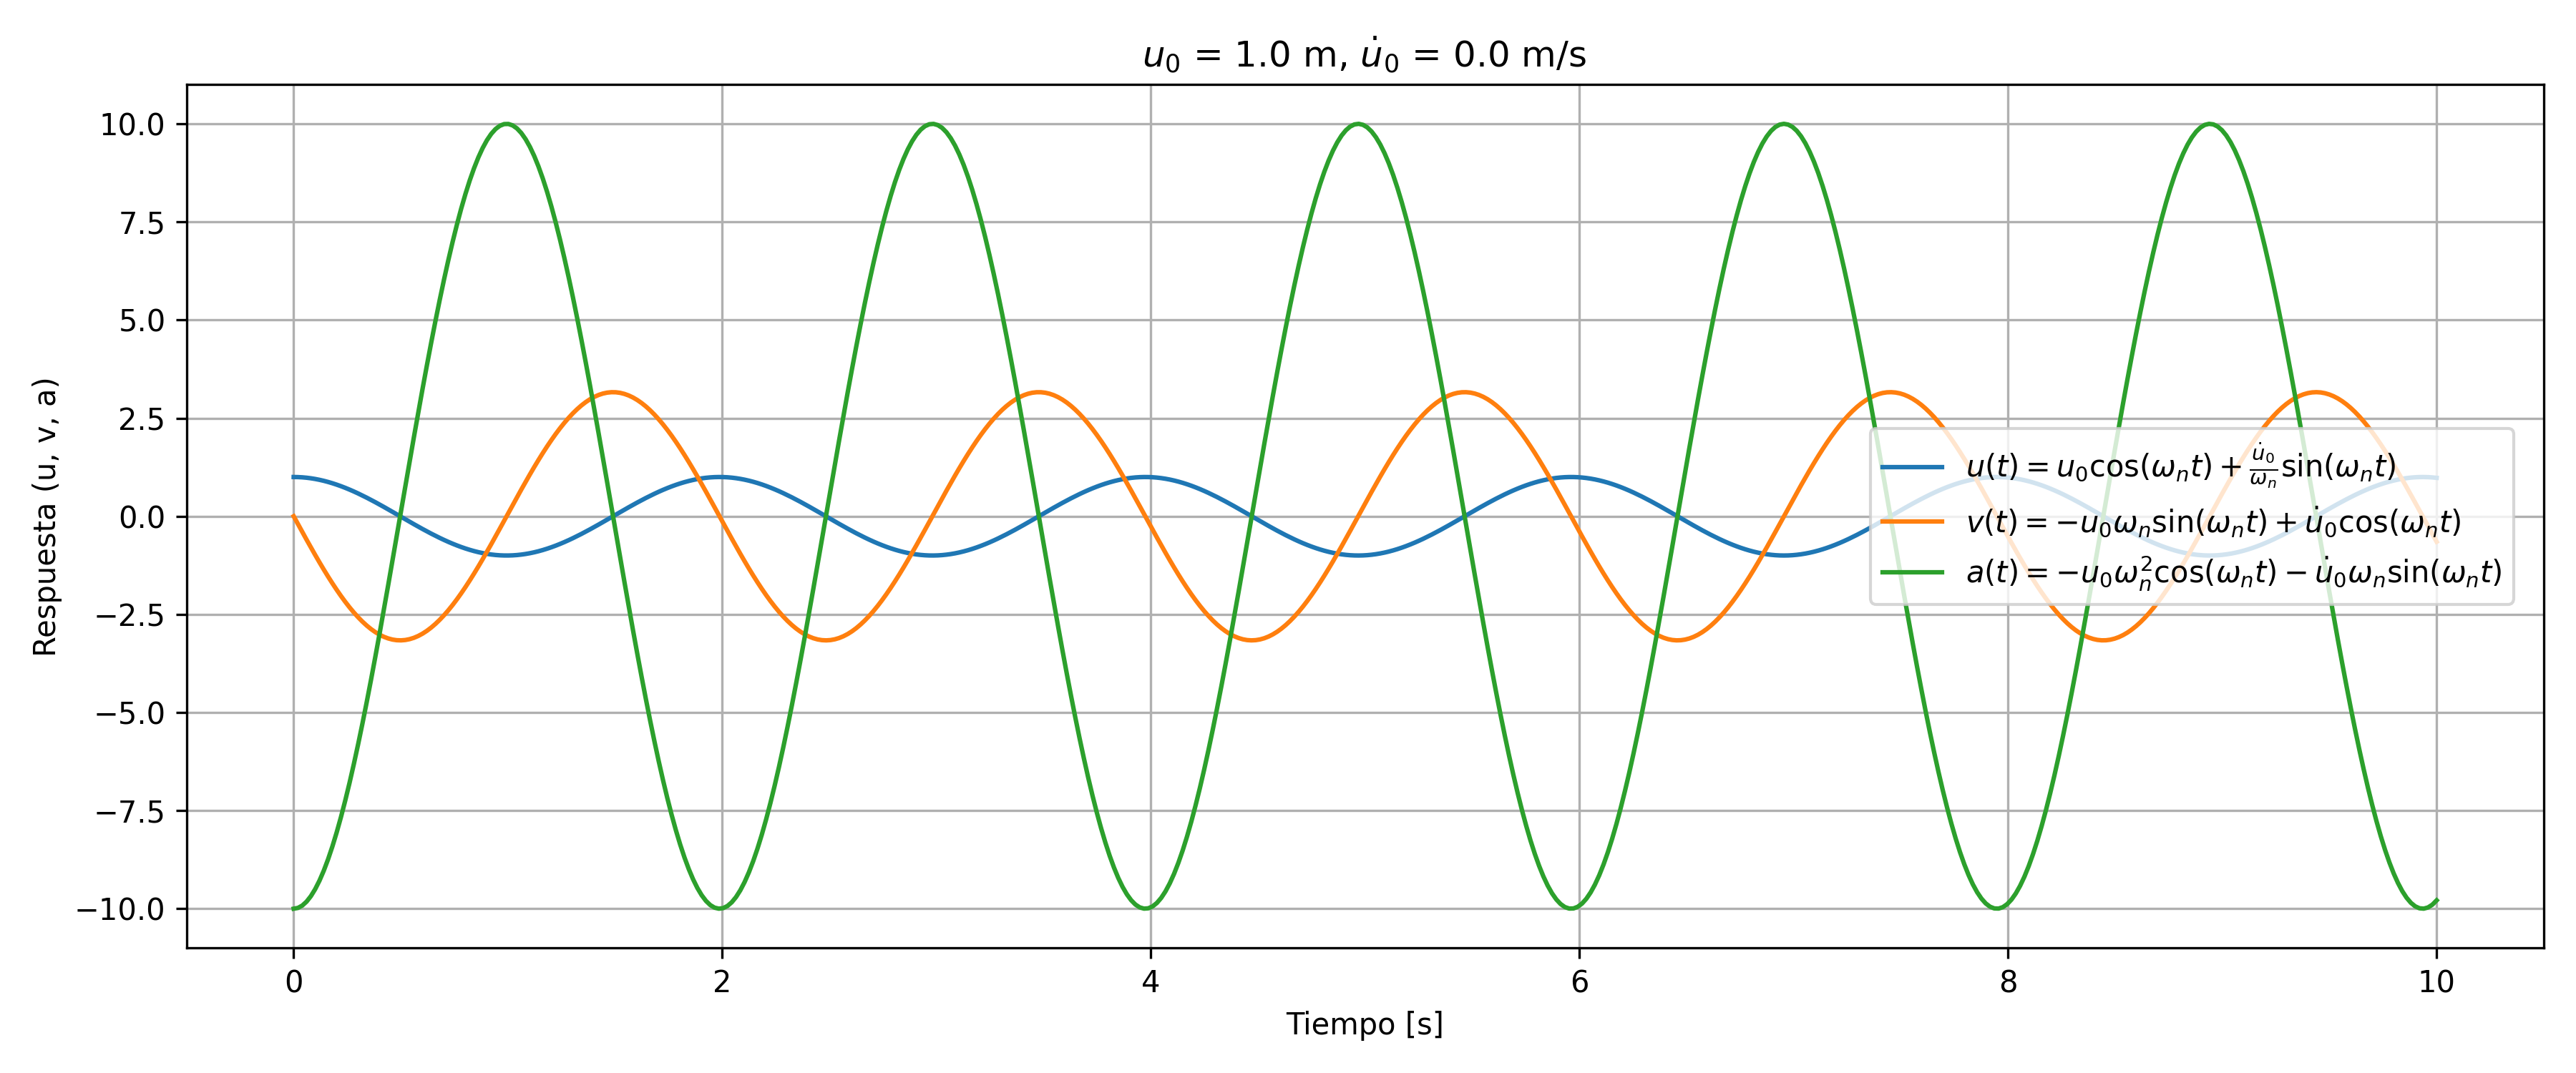
\includegraphics[width=1\textwidth]{GRAFICOS/sis_no_amortiguado_u0_1.0_v0_0.0.png}
    \caption{Desplazamiento inicial 1.0, velocidad inicial 0.0}
    \label{fig:ejemplo1}
\end{figure}

\begin{figure}[H]
    \centering
    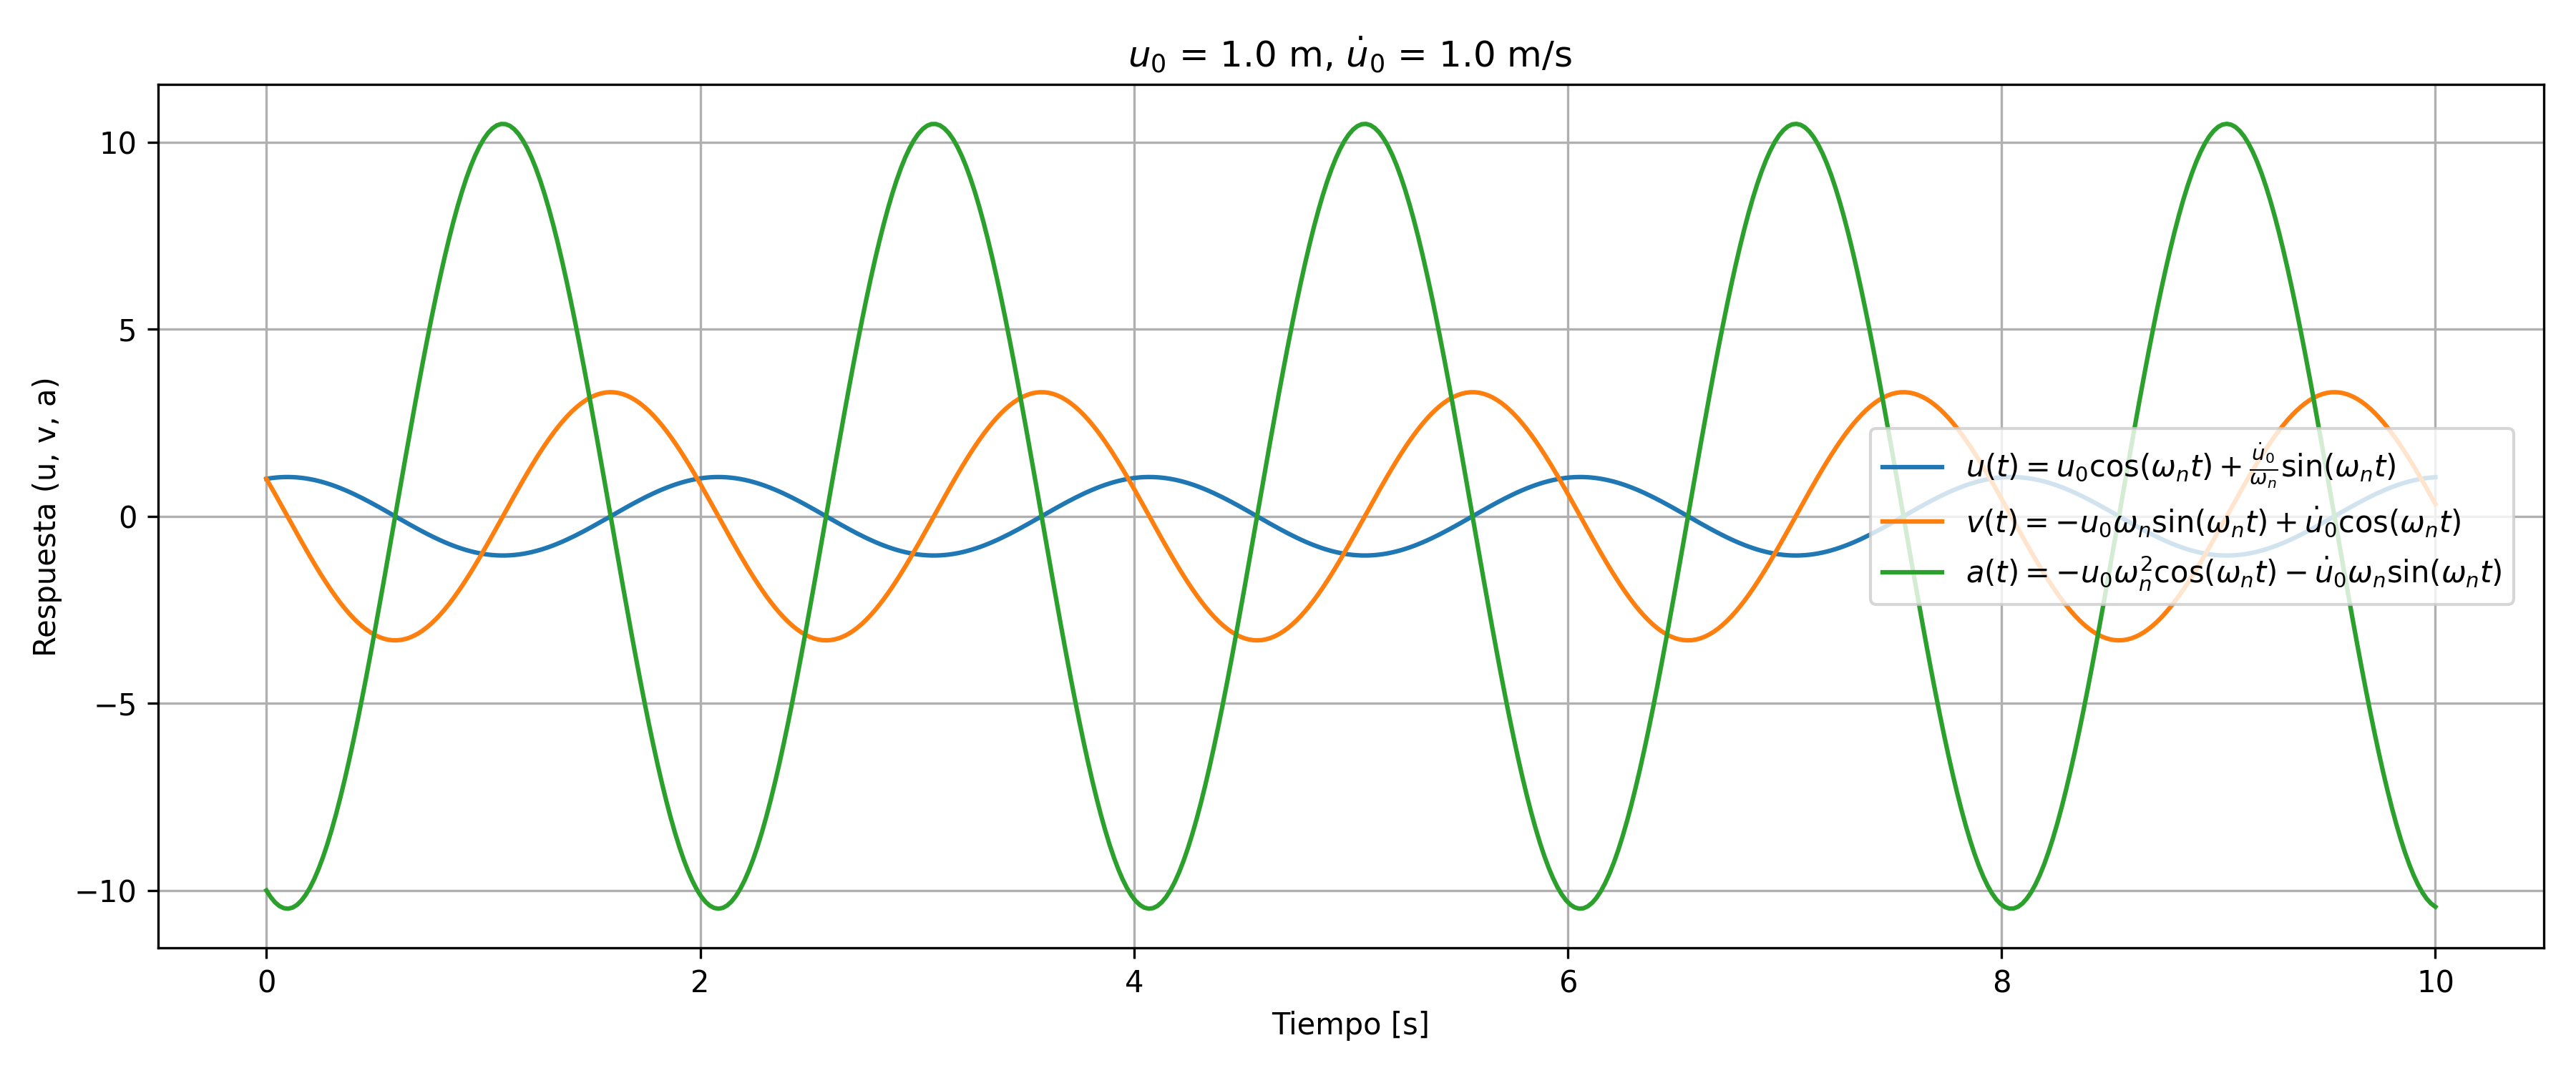
\includegraphics[width=1\textwidth]{GRAFICOS/sis_no_amortiguado_u0_1.0_v0_1.0.png}
    \caption{Desplazamiento inicial 1.0, velocidad inicial 1.0}
    \label{fig:ejemplo1}
\end{figure}

\newpage
\section{Vibraciones Libres Armortiguadas}

Se define la ecuacion de movimiento como:
\begin{equation}
    m \ddot{x} + c \dot{x} + kx = 0
\end{equation}

Luego existen 3 tipos de sistemas:
\begin{itemize}
    \item \textbf{Sobreamortiguado:} $(\frac{c}{2m\omega_n})^2 > 1 \rightarrow S_{1,2} \in \mathbb{R}$ 
    \item \textbf{Criticamente amortiguado:} $(\frac{c}{2m\omega_n})^2 = 1  \rightarrow S_{1,2} = \frac{-c}{2m}$
    \item \textbf{Subamortiguado:} $(\frac{c}{2m\omega_n})^2 < 1 \rightarrow S_{1,2} \in \mathbb{C}$
\end{itemize}

Se define la razon de amortiguamiento critico como:

\begin{equation}
    \beta = \zeta = \frac{c}{c_c} = \frac{c}{2m\omega_n}
\end{equation}

Por lo tanto, la razon de armortiguamiento para los distintos casos es:

\begin{itemize}
    \item \textbf{Sobreamortiguado:} $\beta > 1$
    \item \textbf{Criticamente amortiguado:} $\beta = 1$
    \item \textbf{Subamortiguado:} $\beta < 1$
\end{itemize}

Ademas, se define la frecuencia amortiguada como:

\begin{equation}
    \omega_d = \omega_n \sqrt{\beta^2 - 1} \quad \text{para} \quad \beta >= 1
\end{equation}

\begin{equation}
    \omega_d = \omega_n \sqrt{1 - \beta^2} \quad \text{para} \quad \beta < 1
\end{equation}
\subsection{Sobreamortiguado}

La ecuacion de movimiento se puede escribir como:

\begin{equation}
    u(t) = G_1 e^{-(\beta \omega_n t + \omega_d)t} + G_2 e^{-(\beta \omega_n t - \omega_d)t} \quad G_1, G_2 \in \mathbb{R}
\end{equation}

Lo cual puedo trabajar como:

\begin{equation}
    u(t) = e^{-\beta \omega_n t} (G_1 e^{\omega_d t} + G_2 e^{-\omega_d t}) 
\end{equation}

Luego para graficar hay que considerar las funciones hiperbólicas, donde:

\begin{equation}
    \sinh(\alpha) = \frac{e^{\alpha} - e^{-\alpha}}{2} \quad \text{y} \quad \cosh(\alpha) = \frac{e^{\alpha} + e^{-\alpha}}{2}
\end{equation}

Algunos ejemplos son:

\begin{figure}[H]
    \centering
    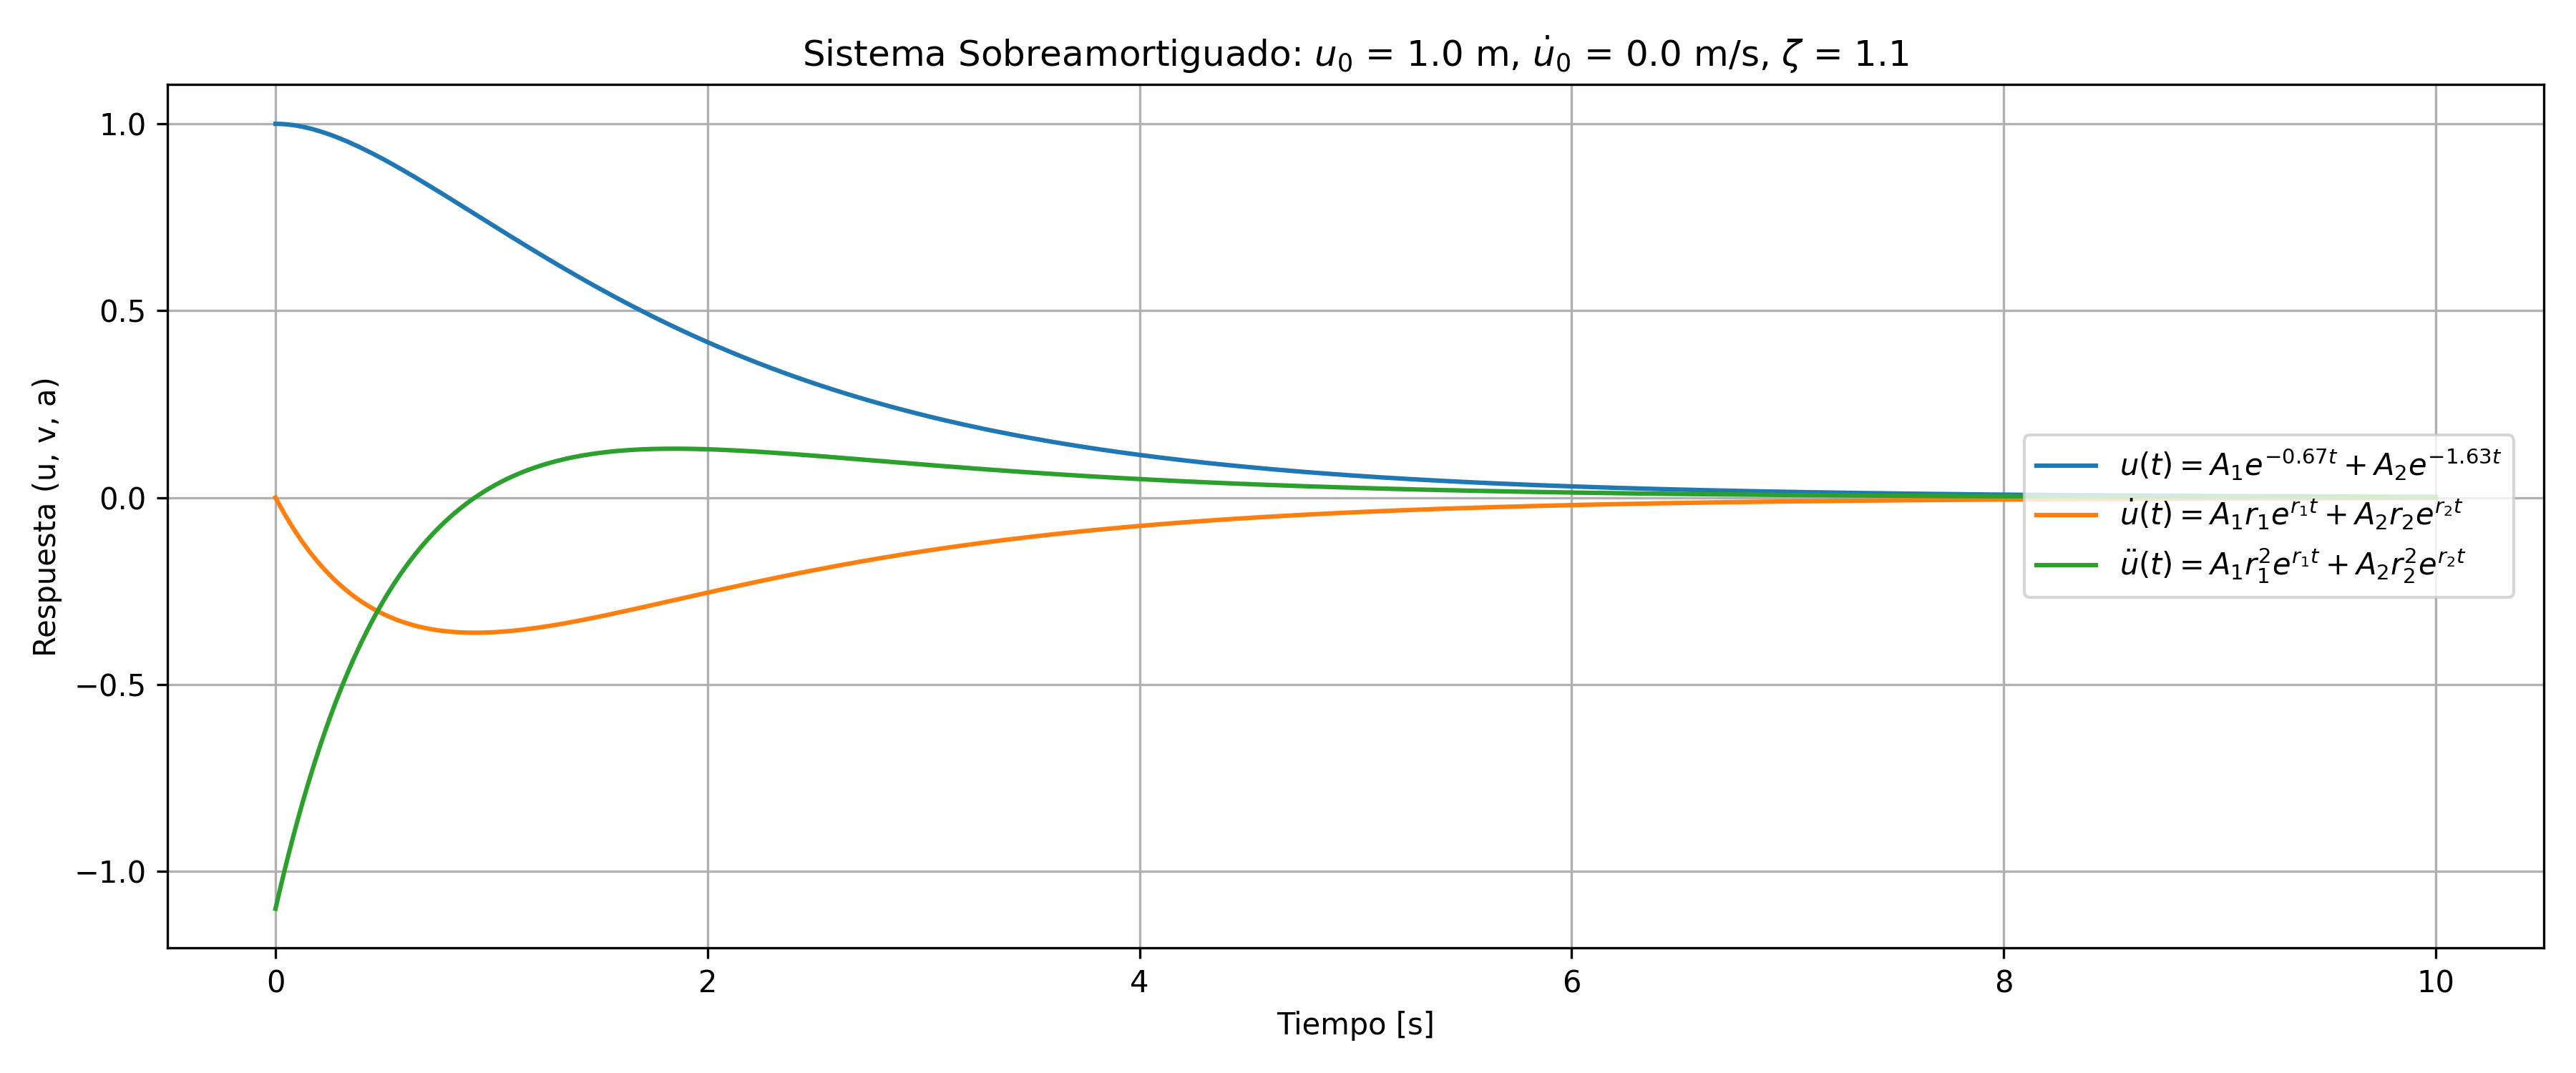
\includegraphics[width=1\textwidth]{GRAFICOS/sis_sobreamortiguado_u0_1.0_v0_0.0_zeta_1.1.png}
    \caption{Desplazamiento inicial 1.0, velocidad inicial 0.0}
    \label{fig:ejemplo1}
\end{figure}

\begin{figure}[H]
    \centering
    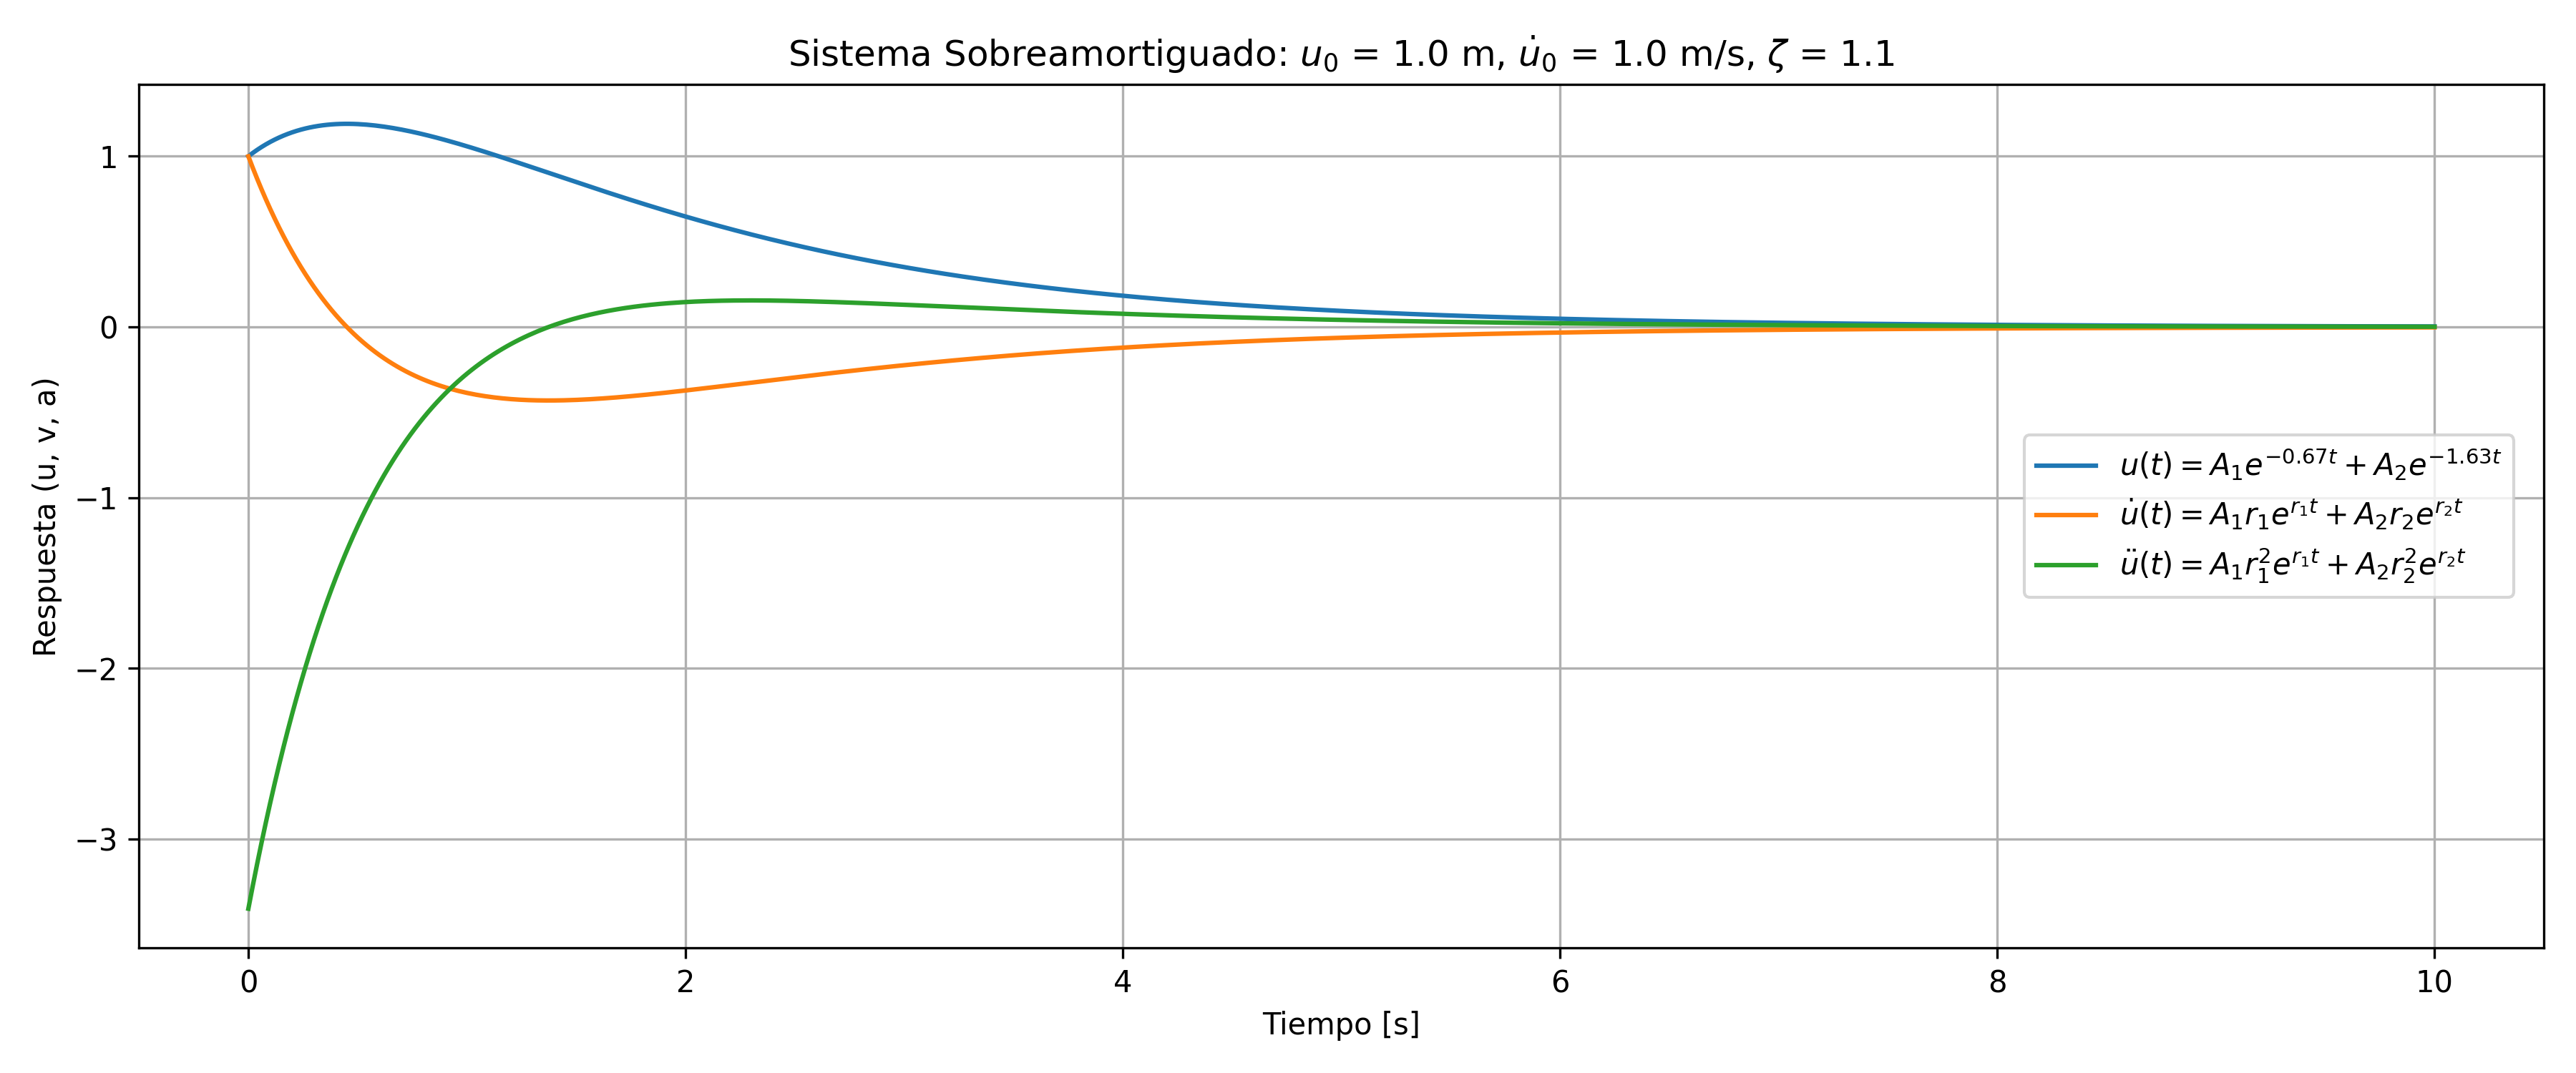
\includegraphics[width=1\textwidth]{GRAFICOS/sis_sobreamortiguado_u0_1.0_v0_1.0_zeta_1.1.png}
    \caption{Desplazamiento inicial 1.0, velocidad inicial 1.0}
    \label{fig:ejemplo1}
\end{figure}

\subsection{Criticamente amortiguado}

Las soluciones a la ecuacion de movimiento son:

\begin{equation}
   S_{1,2} = -\beta \omega_n = \omega_n
\end{equation}

Por lo tanto:

\begin{equation}
    u(t) = G_1e^{-\omega_n t} 
\end{equation}
\begin{equation}
    u_2(t) = G_2e^{-\omega_n t}
\end{equation}

Luego:

\begin{equation}
    u(t) = G_1e^{-\omega_n t} + G_2te^{-\omega_n t} \quad G_1, G_2 \in \mathbb{R}
\end{equation}

Algunos ejemplos son:
\begin{figure}[H]
    \centering
    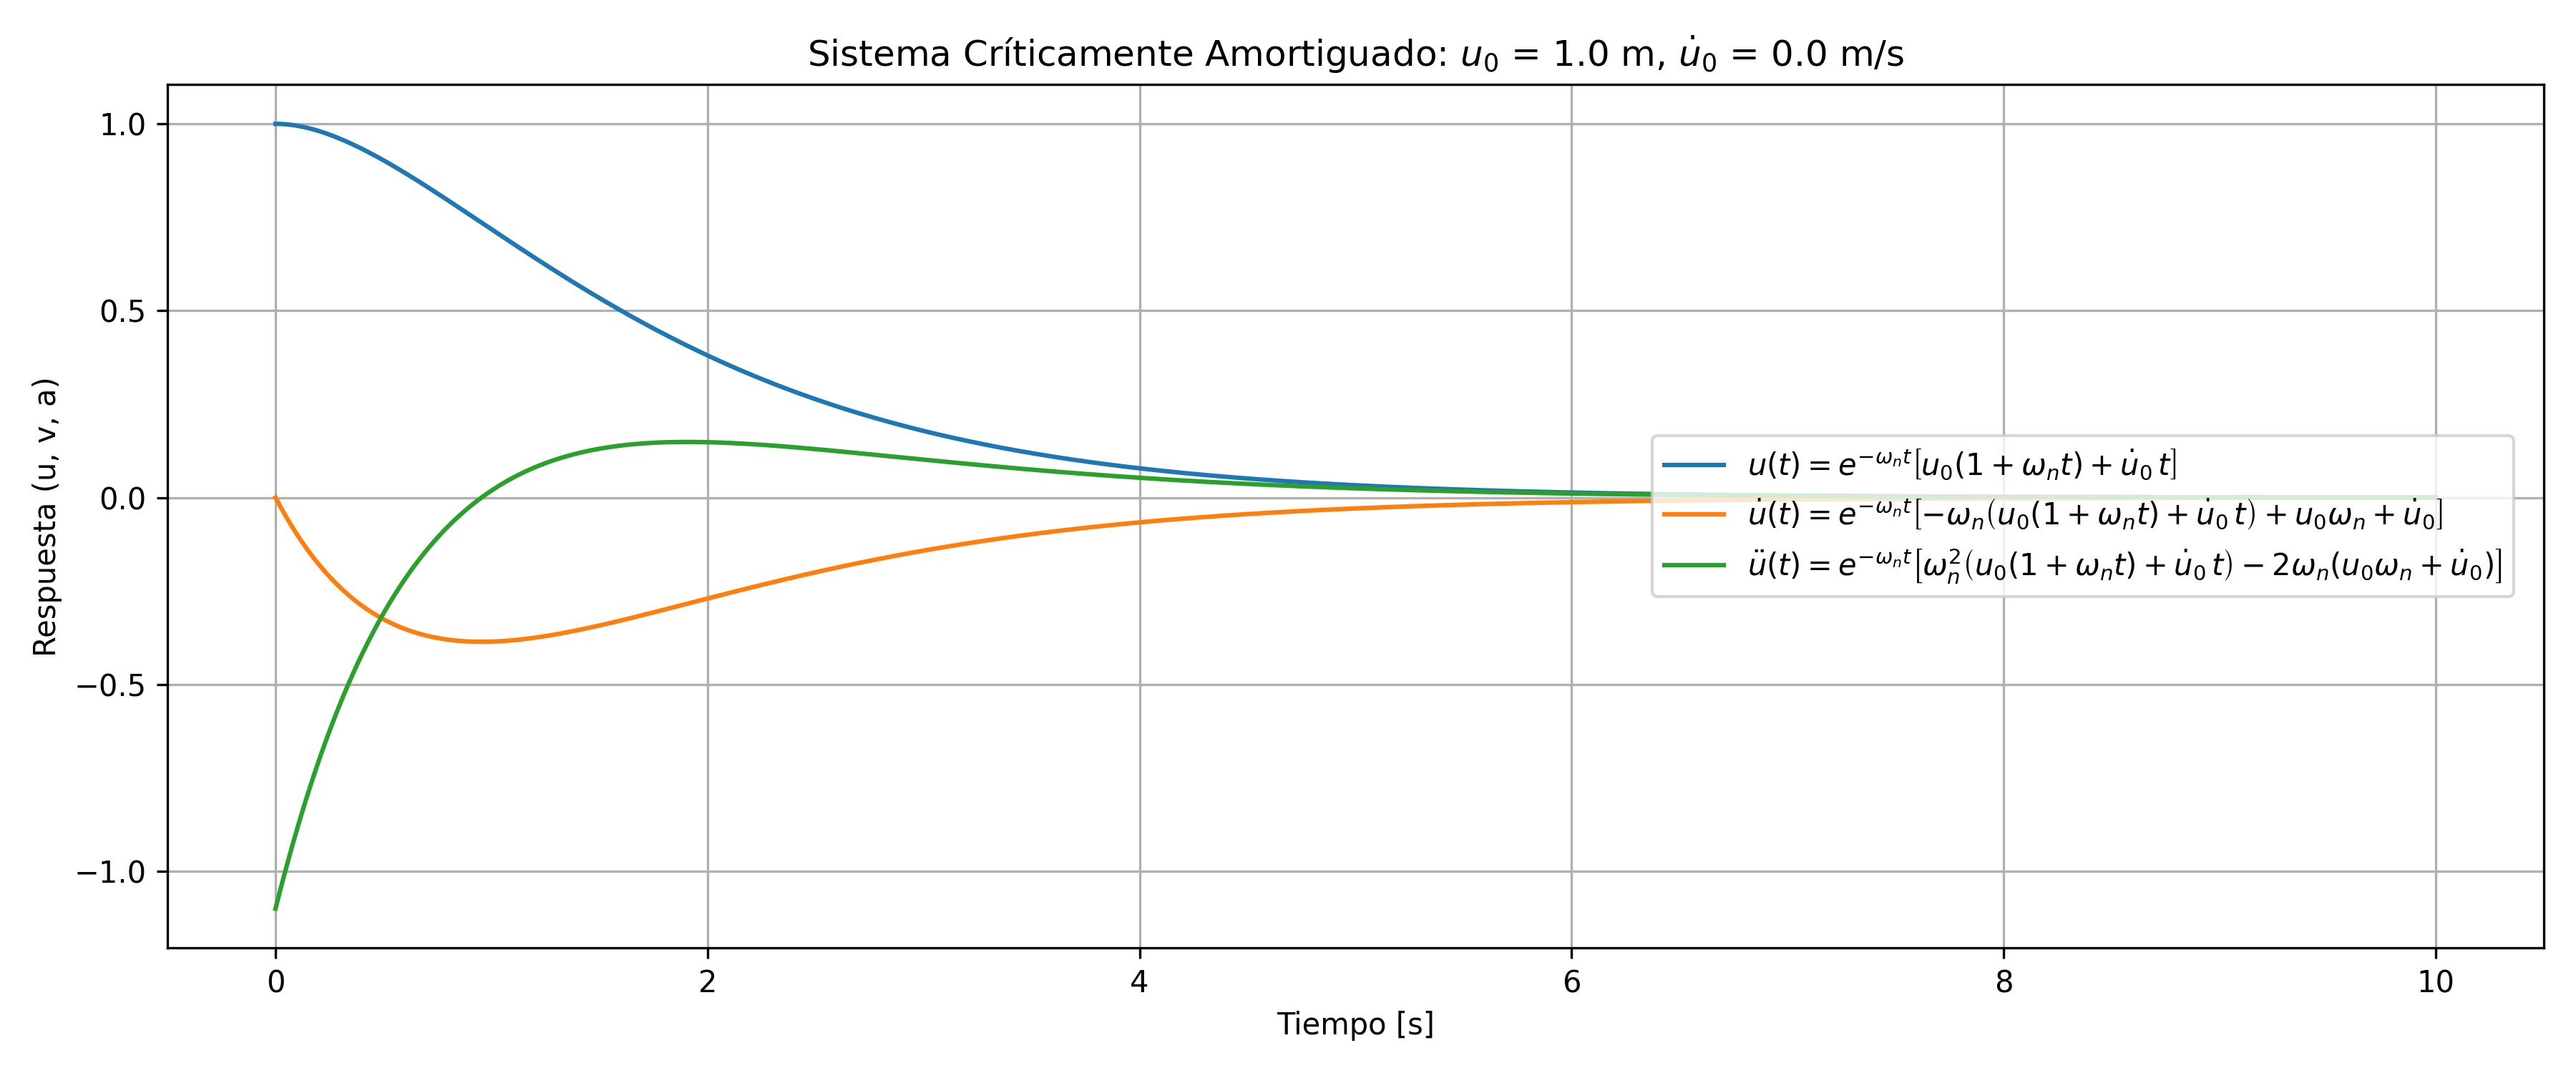
\includegraphics[width=1\textwidth]{GRAFICOS/sis_criticamente_amortiguado_u0_1.0_v0_0.0.png}
    \caption{Desplazamiento inicial 1.0, velocidad inicial 0.0}
    \label{fig:ejemplo1}
\end{figure}

\begin{figure}[H]
    \centering
    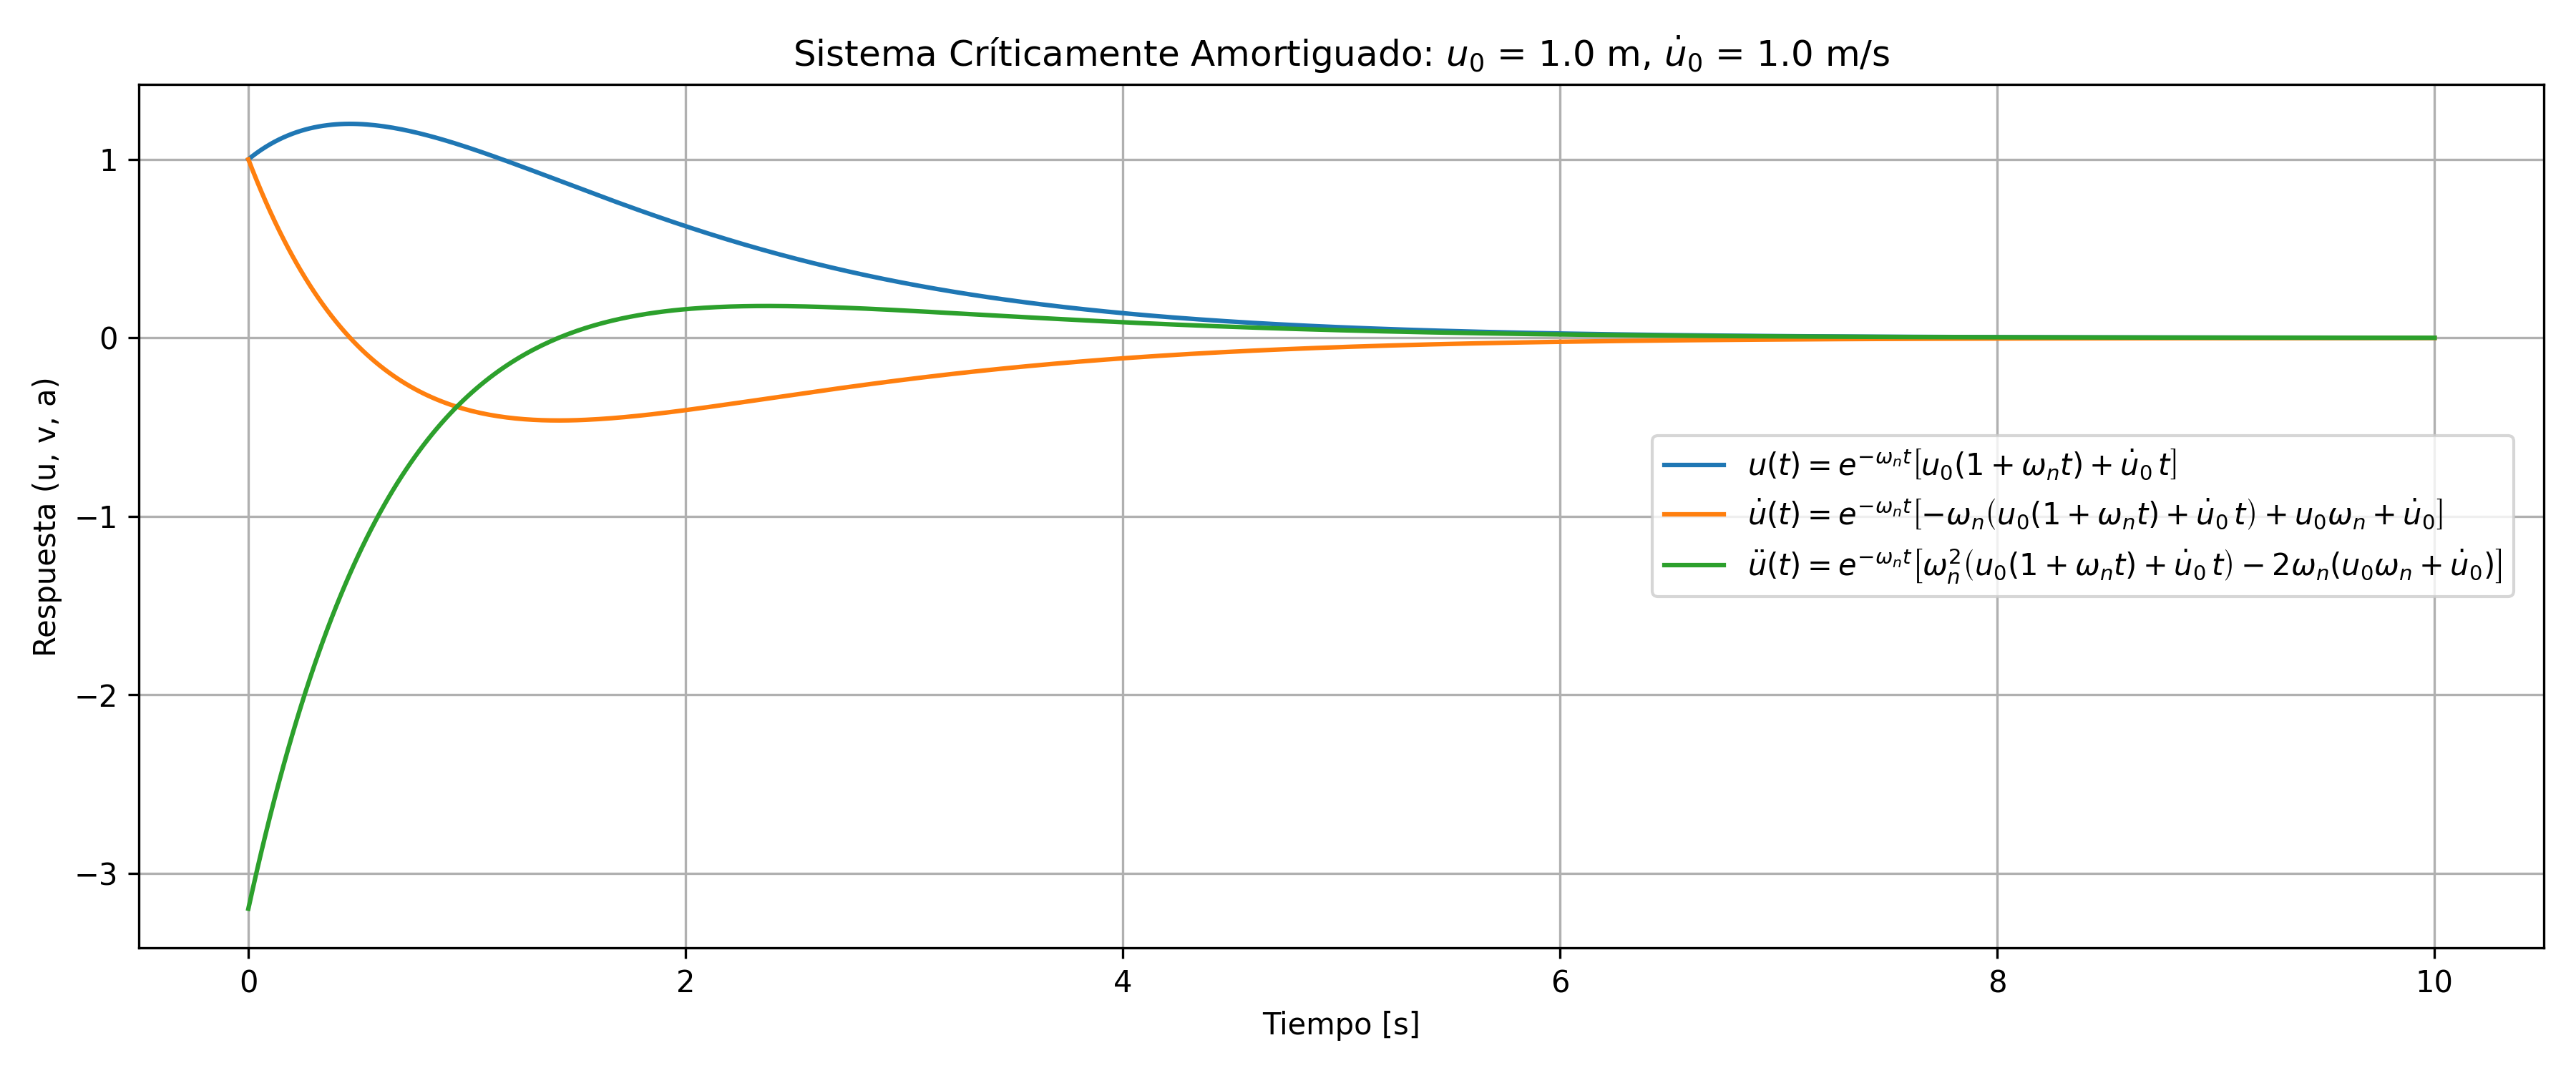
\includegraphics[width=1\textwidth]{GRAFICOS/sis_criticamente_amortiguado_u0_1.0_v0_1.0.png}
    \caption{Desplazamiento inicial 1.0, velocidad inicial 1.0}
    \label{fig:ejemplo1}
\end{figure}

\subsection{Subamortiguado}

Algunos ejemplos son:

\begin{figure}[H]
    \centering
    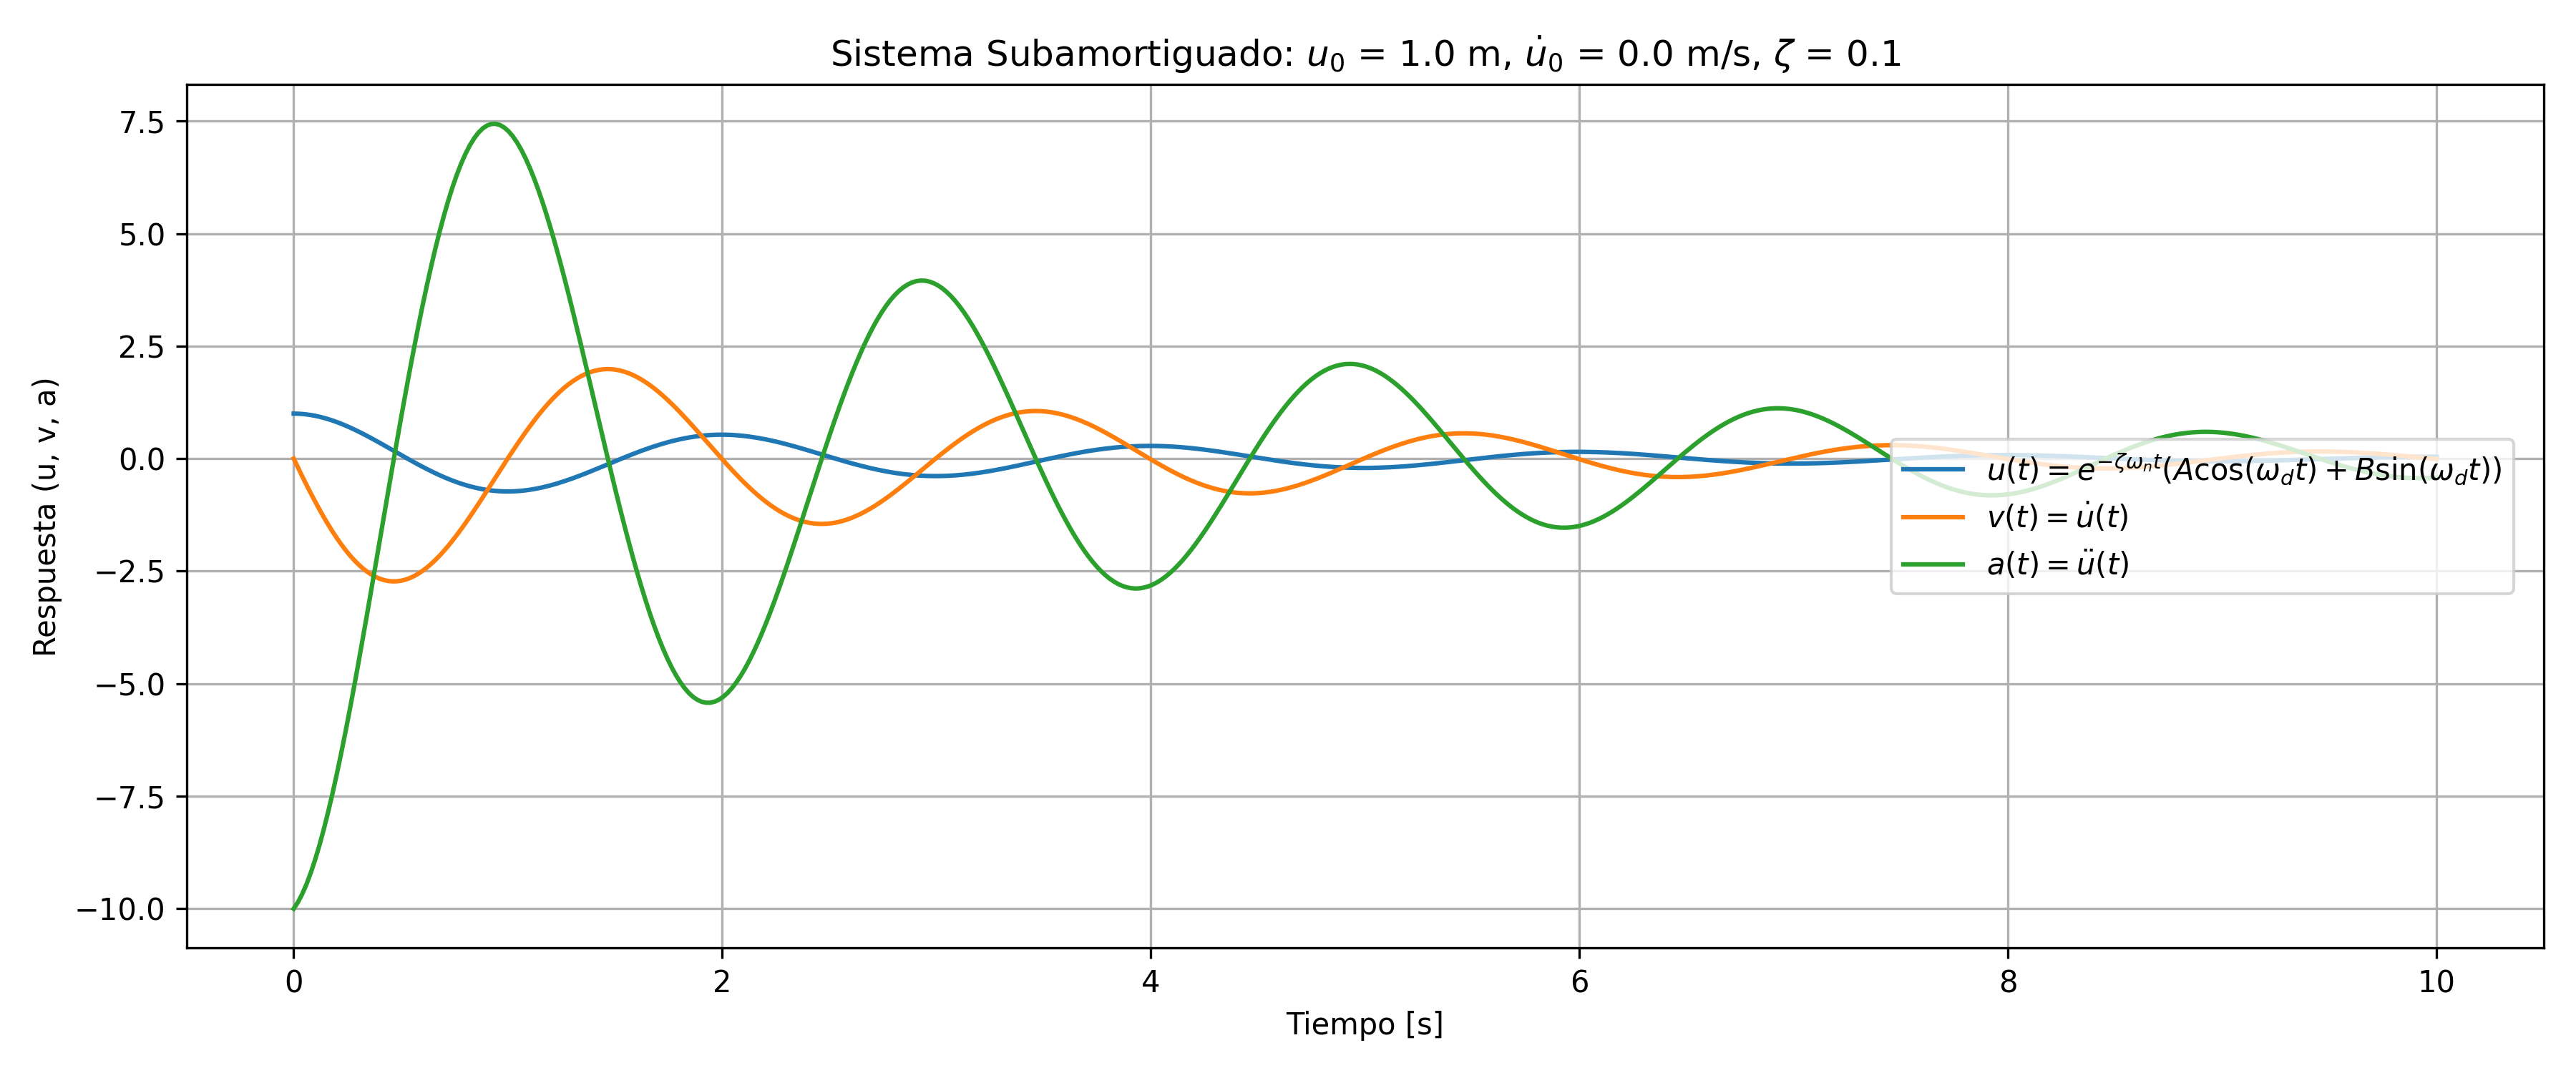
\includegraphics[width=1\textwidth]{GRAFICOS/sis_subamortiguado_u0_1.0_v0_0.0_zeta_0.1.png}
    \caption{Desplazamiento inicial 1.0, velocidad inicial 0.0}
    \label{fig:ejemplo1}
\end{figure}

\begin{figure}[H]
    \centering
    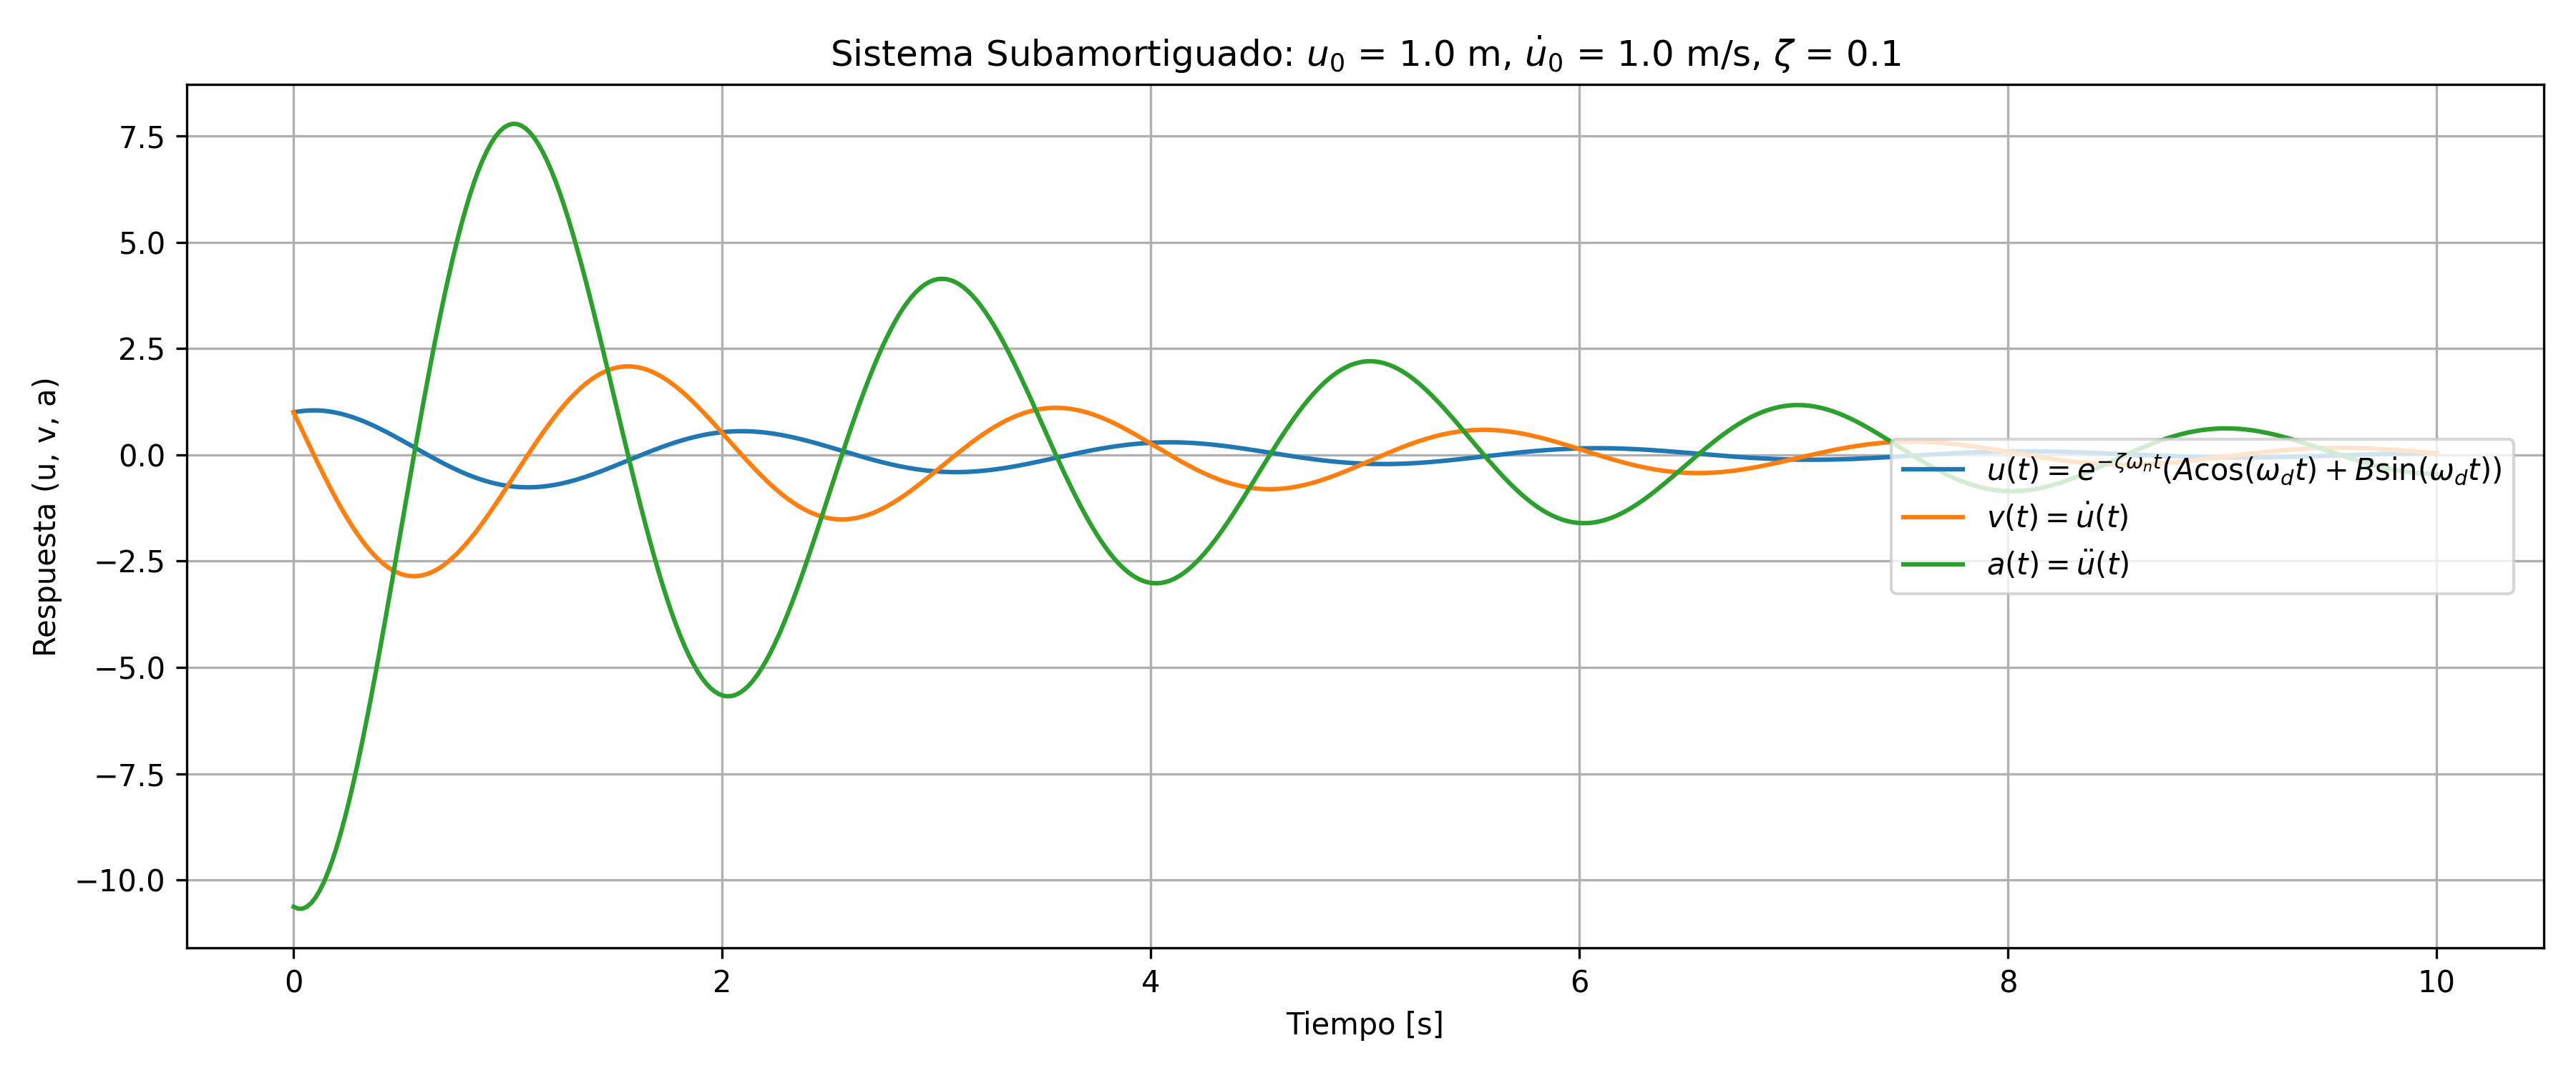
\includegraphics[width=1\textwidth]{GRAFICOS/sis_subamortiguado_u0_1.0_v0_1.0_zeta_0.1.png}
    \caption{Desplazamiento inicial 1.0, velocidad inicial 1.0}
    \label{fig:ejemplo1}
\end{figure}


\end{document}
